\documentclass[aspectratio=169,hyperref={pdfpagelabels=false,colorlinks=true,linkcolor=white,urlcolor=gtgold},t]{beamer}

%%%%%%%%%%%%%%%%%%%%%%%%%%%%%%%%%%%%%%%%%%%%%%%%%%%%%%%%%%%%%%%%%%%%%%%%%%%%%%%%%%
%%%%%%%%%%%%%%%%%%%%%%%%%%%%%%%%%%%%%%%%%%%%%%%%%%%%%%%%%%%%%%%%%%%%%%%%%%%%%%%%%%
% packages
\usepackage{pict2e}
\usepackage{epic}
\usepackage{amsmath,amsfonts,amssymb}
\usepackage{units}
\usepackage{fancybox}
\usepackage[absolute,overlay]{textpos} 
%\usepackage{media9} % avi2flv: "C:\Program Files\ffmpeg\bin\ffmpeg.exe" -i TuneFreqFilterbank.avi -b 600k -s 441x324 -r 15 -acodec copy TuneFreqFilterbank.flv
\usepackage{animate}
\usepackage{gensymb}
\usepackage{multirow}
\usepackage{silence}
\usepackage{tikz}
\usepackage[backend=bibtex,style=ieee]{biblatex}
\AtEveryCitekey{\iffootnote{\tiny}{}}
\addbibresource{include/lerch}



% fontsize
\let\Tiny=\tiny

%%%%%%%%%%%%%%%%%%%%%%%%%%%%%%%%%%%%%%%%%%%%%%%%%%%%%%%%%%%%%%%%%%%%%%%%%%%%%%%%%%
%%%%%%%%%%%%%%%%%%%%%%%%%%%%%%%%%%%%%%%%%%%%%%%%%%%%%%%%%%%%%%%%%%%%%%%%%%%%%%%%%%
% warnings
\pdfsuppresswarningpagegroup=1
\WarningFilter{biblatex}{Patching footnotes failed}
\WarningFilter{latexfont}{Font shape}
\WarningFilter{latexfont}{Some font shapes}
\WarningFilter{gensymb}{Not defining}


%%%%%%%%%%%%%%%%%%%%%%%%%%%%%%%%%%%%%%%%%%%%%%%%%%%%%%%%%%%%%%%%%%%%%%%%%%%%%%%%%%
%%%%%%%%%%%%%%%%%%%%%%%%%%%%%%%%%%%%%%%%%%%%%%%%%%%%%%%%%%%%%%%%%%%%%%%%%%%%%%%%%%
% theme & layout
\usetheme{Frankfurt}
\useinnertheme{rectangles}


%%%%%%%%%%%%%%%%%%%%%%%%%%%%%%%%%%%%%%%%%%%%%%%%%%%%%%%%%%%%%%%%%%%%%%%%%%%%%%%%%%
\setbeamertemplate{frametitle}[default][colsep=-4bp,rounded=false,shadow=false]
\setbeamertemplate{frametitle}
{%
    \nointerlineskip%
    %\vskip-0.5ex
    \begin{beamercolorbox}[wd=\paperwidth,ht=3.5ex,dp=0.6ex]{frametitle}
        \hspace*{1.3ex}\insertframetitle%
        
        \hspace*{1.3ex}\small\insertframesubtitle%
    \end{beamercolorbox}%
    \begin{textblock*}{100mm}(11.6cm,.57cm)
        
\includegraphics[height=.8cm,keepaspectratio]{graph/Logo_GTCMT_white}
    \end{textblock*}
}


%%%%%%%%%%%%%%%%%%%%%%%%%%%%%%%%%%%%%%%%%%%%%%%%%%%%%%%%%%%%%%%%%%%%%%%%%%%%%%%%%%
\setbeamertemplate{title page}[default][colsep=-4bp,rounded=false,shadow=false]
\setbeamertemplate{title page}
{
    \begin{textblock*}{200mm}(13.5cm,.5cm)
            \href{https://www.\repolink}{
\includegraphics[height=2cm,keepaspectratio]{graph/qr}}\hspace*{2ex}
    \end{textblock*}
    \vskip-10ex
    \begin{beamercolorbox}[wd=\paperwidth,ht=.7\paperheight,dp=0.6ex]{frametitle} %35ex
        \hspace*{1.8ex}\LARGE\inserttitle%
        
        \vspace*{.5ex}
        
        \hspace*{1.3ex}\small\insertsubtitle%
        
        \vspace*{.5ex}
    \end{beamercolorbox}%
    \nointerlineskip%
    \begin{beamercolorbox}[wd=\paperwidth,ht=.4\paperheight,dp=0.6ex]{page number in head/foot}
        %\vspace*{-.5ex}
        \hspace*{1.7ex}\small\insertauthor%
        
        %\hspace*{1.7ex}\small }%
        
        \vspace*{10ex}
        
        \begin{flushright}
            \href{http://www.gtcmt.gatech.edu}{
\includegraphics[height=.8cm,keepaspectratio]{graph/Logo_GTCMT_black}}\hspace*{2ex}
        \end{flushright}
    \end{beamercolorbox}%
    \nointerlineskip%
    \begin{beamercolorbox}[wd=\paperwidth,ht=.2\paperheight,dp=0.6ex]{page number in head/foot}
    \end{beamercolorbox}%
	\addreference{\hspace{48mm}\href{https://\repolink}{\repolink}}
}


%%%%%%%%%%%%%%%%%%%%%%%%%%%%%%%%%%%%%%%%%%%%%%%%%%%%%%%%%%%%%%%%%%%%%%%%%%%%%%%%%%
%\makeatother
\setbeamertemplate{footline}
{
  \leavevmode%
  \hbox{%
  \begin{beamercolorbox}[wd=.5\paperwidth,ht=2.25ex,dp=1ex,left,leftskip=1ex]{page number in head/foot}%
    \inserttitle
  \end{beamercolorbox}%
  \begin{beamercolorbox}[wd=.5\paperwidth,ht=2.25ex,dp=1ex,right,rightskip=1ex]{page number in head/foot}%
    \hfill
    \insertframenumber{} / \inserttotalframenumber
  \end{beamercolorbox}}%
  \vskip0pt%
}
%\makeatletter


%%%%%%%%%%%%%%%%%%%%%%%%%%%%%%%%%%%%%%%%%%%%%%%%%%%%%%%%%%%%%%%%%%%%%%%%%%%%%%%%%%
\beamertemplatenavigationsymbolsempty
\setbeamertemplate{navigation symbols}{}
\setbeamertemplate{blocks}[default]%[rounded=false,shadow=false]
\setbeamertemplate{itemize item}[square]
\setbeamertemplate{itemize subitem}[circle]
\setbeamertemplate{itemize subsubitem}[triangle]
\setbeamertemplate{enumerate item}[square]
\setbeamertemplate{enumerate subitem}[circle]
\setbeamertemplate{enumerate subsubitem}[circle]
%\setbeamertemplate{section in toc}[default]

%%%%%%%%%%%%%%%%%%%%%%%%%%%%%%%%%%%%%%%%%%%%%%%%%%%%%%%%%%%%%%%%%%%%%%%%%%%%%%%%%%
% colors
\setbeamercolor{structure}{fg=darkgray}
\setbeamercovered{transparent} %invisible
\setbeamercolor{bibliography entry author}{fg=black}
\setbeamercolor*{bibliography entry title}{fg=black}
\setbeamercolor*{bibliography entry note}{fg=black}
\setbeamercolor{frametitle}{fg=black}
\setbeamercolor{title}{fg=white}
\setbeamercolor{subtitle}{fg=white}
\setbeamercolor{frametitle}{fg=white}
\setbeamercolor{framesubtitle}{fg=white}
\setbeamercolor{mini frame}{fg=white, bg=black}
\setbeamercolor{section in head/foot}{fg=white, bg=darkgray}
\setbeamercolor{page number in head/foot}{fg=black, bg=gtgold}
\setbeamercolor{item projected}{fg=white, bg=black}
\setbeamercolor{section in toc}{fg=black, bg=gtgold}
\setbeamercolor{subsection in toc}{fg=darkgray, bg=gtgold}
%---------------------------------------------------------------------------------
%%%%%%%%%%%%%%%%%%%%%%%%%%%%%%%%%%%%%%%%%%%%%%%%%%%%%%%%%%%%%%%%%%%%%%%%%%%%%%%%%%
%%%%%%%%%%%%%%%%%%%%%%%%%%%%%%%%%%%%%%%%%%%%%%%%%%%%%%%%%%%%%%%%%%%%%%%%%%%%%%%%%%
% title information
\title[]{Introduction to Audio Content Analysis}   
\author[alexander lerch]{alexander lerch} 
%\institute{~}
%\date[Alexander Lerch]{}
%\titlegraphic{\vspace{-16mm}\includegraphics[width=\textwidth,height=3cm]{title}}

%%%%%%%%%%%%%%%%%%%%%%%%%%%%%%%%%%%%%%%%%%%%%%%%%%%%%%%%%%%%%%%%%%%%%%%%%%%%%%%%%%
%%%%%%%%%%%%%%%%%%%%%%%%%%%%%%%%%%%%%%%%%%%%%%%%%%%%%%%%%%%%%%%%%%%%%%%%%%%%%%%%%%
% colors
\definecolor{gtgold}{HTML}{E0AA0F} %{rgb}{0.88,0.66,1,0.06} [234, 170, 0]/256
\definecolor{darkgray}{rgb}{.2,.2,.2}
%\definecolor{gtgold_less}{rgb}{.88,0.66,0} %_less!40

%%%%%%%%%%%%%%%%%%%%%%%%%%%%%%%%%%%%%%%%%%%%%%%%%%%%%%%%%%%%%%%%%%%%%%%%%%%%%%%%%%
%%%%%%%%%%%%%%%%%%%%%%%%%%%%%%%%%%%%%%%%%%%%%%%%%%%%%%%%%%%%%%%%%%%%%%%%%%%%%%%%%%
% relative paths
\graphicspath{{./graph/}}

%%%%%%%%%%%%%%%%%%%%%%%%%%%%%%%%%%%%%%%%%%%%%%%%%%%%%%%%%%%%%%%%%%%%%%%%%%%%%%%%%%
%%%%%%%%%%%%%%%%%%%%%%%%%%%%%%%%%%%%%%%%%%%%%%%%%%%%%%%%%%%%%%%%%%%%%%%%%%%%%%%%%%
% links
\def\repolink{github.com/alexanderlerch/\jobname}


%%%%%%%%%%%%%%%%%%%%%%%%%%%%%%%%%%%%%%%%%%%%%%%%%%%%%%%%%%%%%%%%%%%%%%%%%%%%%%%%%%
%%%%%%%%%%%%%%%%%%%%%%%%%%%%%%%%%%%%%%%%%%%%%%%%%%%%%%%%%%%%%%%%%%%%%%%%%%%%%%%%%%
% units
\setlength{\unitlength}{1mm}

%%%%%%%%%%%%%%%%%%%%%%%%%%%%%%%%%%%%%%%%%%%%%%%%%%%%%%%%%%%%%%%%%%%%%%%%%%%%%%%%%%
%%%%%%%%%%%%%%%%%%%%%%%%%%%%%%%%%%%%%%%%%%%%%%%%%%%%%%%%%%%%%%%%%%%%%%%%%%%%%%%%%%
% math
\DeclareMathOperator*{\argmax}{argmax}
\DeclareMathOperator*{\argmin}{argmin}
\DeclareMathOperator*{\atan}{atan}
\DeclareMathOperator*{\arcsinh}{arcsinh}
\DeclareMathOperator*{\sign}{sign}
\DeclareMathOperator*{\tcdf}{tcdf}
\DeclareMathOperator*{\si}{sinc}
\DeclareMathOperator*{\princarg}{princarg}
\DeclareMathOperator*{\arccosh}{arccosh}
\DeclareMathOperator*{\hwr}{HWR}
\DeclareMathOperator*{\flip}{flip}
\DeclareMathOperator*{\sinc}{sinc}
\DeclareMathOperator*{\floor}{floor}
\newcommand{\e}{{e}}
\newcommand{\jom}{\mathrm{j}\omega}
\newcommand{\jOm}{\mathrm{j}\Omega}
\newcommand   {\mat}[1]    		{\boldsymbol{\uppercase{#1}}}		%bold
\renewcommand {\vec}[1]    		{\boldsymbol{\lowercase{#1}}}		%bold

%%%%%%%%%%%%%%%%%%%%%%%%%%%%%%%%%%%%%%%%%%%%%%%%%%%%%%%%%%%%%%%%%%%%%%%%%%%%%%%%%%
%%%%%%%%%%%%%%%%%%%%%%%%%%%%%%%%%%%%%%%%%%%%%%%%%%%%%%%%%%%%%%%%%%%%%%%%%%%%%%%%%%
% media9
\newcommand{\includeaudio}[1]{
\href{run:audio/#1.mp3}{\includegraphics[width=5mm, height=5mm]{graph/SpeakerIcon}}
}
\newcommand{\includevideo}[1]{
\href{run:video/#1}{\includegraphics[width=20mm, height=20mm]{graph/play_button}}
}

\newcommand{\includeanimation}[4]{{\begin{center}
                        \animategraphics[autoplay,loop,scale=.7]{#4}{animation/#1-}{#2}{#3}        
                        \end{center}
                        \addreference{matlab source: \href{https://github.com/alexanderlerch/ACA-Plots/blob/master/matlab/animate#1.m}{matlab/animate#1.m}}}
                        \inserticon{video}}
                        
%%%%%%%%%%%%%%%%%%%%%%%%%%%%%%%%%%%%%%%%%%%%%%%%%%%%%%%%%%%%%%%%%%%%%%%%%%%%%%%%%%
%%%%%%%%%%%%%%%%%%%%%%%%%%%%%%%%%%%%%%%%%%%%%%%%%%%%%%%%%%%%%%%%%%%%%%%%%%%%%%%%%%
% other commands
\newcommand{\question}[1]{%\vspace{-4mm}
                          \setbeamercovered{invisible}
                          \begin{columns}[T]
                            \column{.9\textwidth}
                                \textbf{#1}
                            \column{.1\textwidth}
                                \vspace{-8mm}
                                \begin{flushright}
                                     \includegraphics[width=\columnwidth]{graph/question_mark}
                                \end{flushright}
                                \vspace{6mm}
                          \end{columns}\pause\vspace{-12mm}}

\newcommand{\toremember}[1]{%\vspace{-4mm}
                          %\begin{columns}[T]
                            %\column{.8\textwidth}
                                %\textbf{#1}
                            %\column{.2\textwidth}
                                %\vspace{-4mm}
                                %\begin{flushright}
                                     %\includegraphics[scale=.5]{exclamation_mark}
                                %\end{flushright}
                                %\vspace{6mm}
                          %\end{columns}\vspace{-6mm}
                        \inserticon{lightbulb}
                        }

\newcommand{\matlabexercise}[1]{%\vspace{-4mm}
                          \setbeamercovered{invisible}
                          \begin{columns}[T]
                            \column{.8\textwidth}
                                \textbf{matlab exercise}: #1
                            \column{.2\textwidth}
                                \begin{flushright}
                                     \includegraphics[scale=.5]{graph/logo_matlab}
                                \end{flushright}
                                %\vspace{6mm}
                          \end{columns}}

\newcommand{\addreference}[1]{  
                  
                    \begin{textblock*}{\baselineskip }(.98\paperwidth,.5\textheight) %(1.15\textwidth,.4\textheight)
                         \begin{minipage}[b][.5\paperheight][b]{1cm}%
                            \vfill%
                             \rotatebox{90}{\tiny {#1}}
                        \end{minipage}
                   \end{textblock*}
                    }
                    
\newcommand{\figwithmatlab}[1]{
                    \begin{figure}
                        \centering
                        \includegraphics[scale=.7]{#1}
                        %\label{fig:#1}
                    \end{figure}
                    
                    \addreference{matlab source: \href{https://github.com/alexanderlerch/ACA-Plots/blob/main/matlab/plot#1.m}{plot#1.m}}}
\newcommand{\figwithref}[2]{
                    \begin{figure}
                        \centering
                        \includegraphics[scale=.7]{#1}
                        \label{fig:#1}
                    \end{figure}
                    
                    \addreference{#2}}  
                                    
\newcommand{\inserticon}[1]{

                    \begin{textblock*}{100mm}(14.5cm,7.5cm)
                        \includegraphics[height=.8cm,keepaspectratio]{graph/#1}
                    \end{textblock*}}            

%%%%%%%%%%%%%%%%%%%%%%%%%%%%%%%%%%%%%%%%%%%%%%%%%%%%%%%%%%%%%%%%%%%%%%%%%%%%%%%%%%
%%%%%%%%%%%%%%%%%%%%%%%%%%%%%%%%%%%%%%%%%%%%%%%%%%%%%%%%%%%%%%%%%%%%%%%%%%%%%%%%%%
% counters
\newcounter{i}
\newcounter{j}
\newcounter{iXOffset}
\newcounter{iYOffset}
\newcounter{iXBlockSize}
\newcounter{iYBlockSize}
\newcounter{iYBlockSizeDiv2}
\newcounter{iXBlockSizeDiv2}
\newcounter{iDistance}


\usepackage{multirow}
\AtBeginBibliography{\tiny}

\title{music informatics group}
\subtitle{overview} 

%%%%%%%%%%%%%%%%%%%%%%%%%%%%%%%%%%%%%%%%%%%%%%%%%%%%%%%%%%%%%%%%%%%%%%%%%%%%
\begin{document}
    % generate title page
	{
\setbeamertemplate{headline}{} 
\setbeamertemplate{footline}{} 
\begin{frame}
    \titlepage
    %\vspace{-5mm}
\end{frame}
}
\addtocounter{framenumber}{-1}


    \section[about]{about music informatics group}
        %\input{dolby}
        \begin{frame}{about}{self-introduction}
    \begin{itemize}
        \item   \textbf{education}
            \begin{itemize}
                \item   Electrical Engineering (Technical University Berlin)
                \item   Tonmeister (music production, University of Arts Berlin)
            \end{itemize}
        \bigskip
        \item   \textbf{professional}
            \begin{itemize}
                \item   Associate Professor at the \href{https://music.gatech.edu}{School of Music, Georgia Institute of Technology}
                \item   2000-2013: Head of Research at \href{https://www.zplane.de}{zplane.development}
            \end{itemize}
        \bigskip
        \item   \textbf{background}
            \begin{itemize}
                \item   audio algorithm design (20+ years)
                %\item   classical musician (20+ years)
                \item   commercial music software development (10+ years)
                \item   entrepreneurship (10+ years)
            \end{itemize}
    \end{itemize}
    
    \addreference{\href{https://www.linkedin.com/in/lerch}{www.linkedin.com/in/lerch}}
    %\inserticon{person}
    \vspace{-30mm}
    \begin{flushright}
                            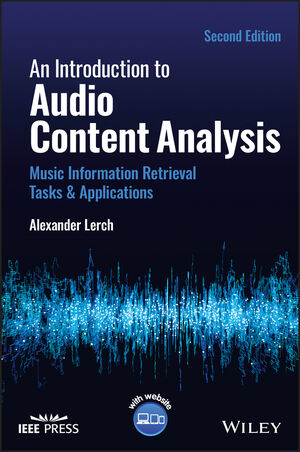
\includegraphics[scale=.20]{cover_aca2_thumb}
    \end{flushright}

\end{frame}

\begin{frame}{introduction}{music informatics group}
    \vspace{-5mm}
    \begin{columns}
    \column{.6\linewidth}
    \begin{itemize}
        %\item   \textbf{research focus}
            %\begin{itemize}
                %\item   machine learning and intelligent DSP solutions for (musical) audio 
            %\end{itemize}
        %\bigskip
        \item   \textbf{mission}
            \begin{itemize}
                \item   create new technologies transforming and improving how we \textit{make, produce, perform, discover, and consume music}
                \item   advance the field of AI for audio through \textit{informed, knowledge-driven machine learning}
            \end{itemize}
        \bigskip
        \item   \textbf{objectives}
            \begin{itemize}
                \item   enable/improve \textit{machine understanding of music} and musical language
                \item   create \textit{interpretable and controllable systems}
                \item   design algorithms with \textit{low data requirements}
            \end{itemize}
    \end{itemize}
    \column{.4\linewidth}
        \vspace{12mm}\begin{figure}%
            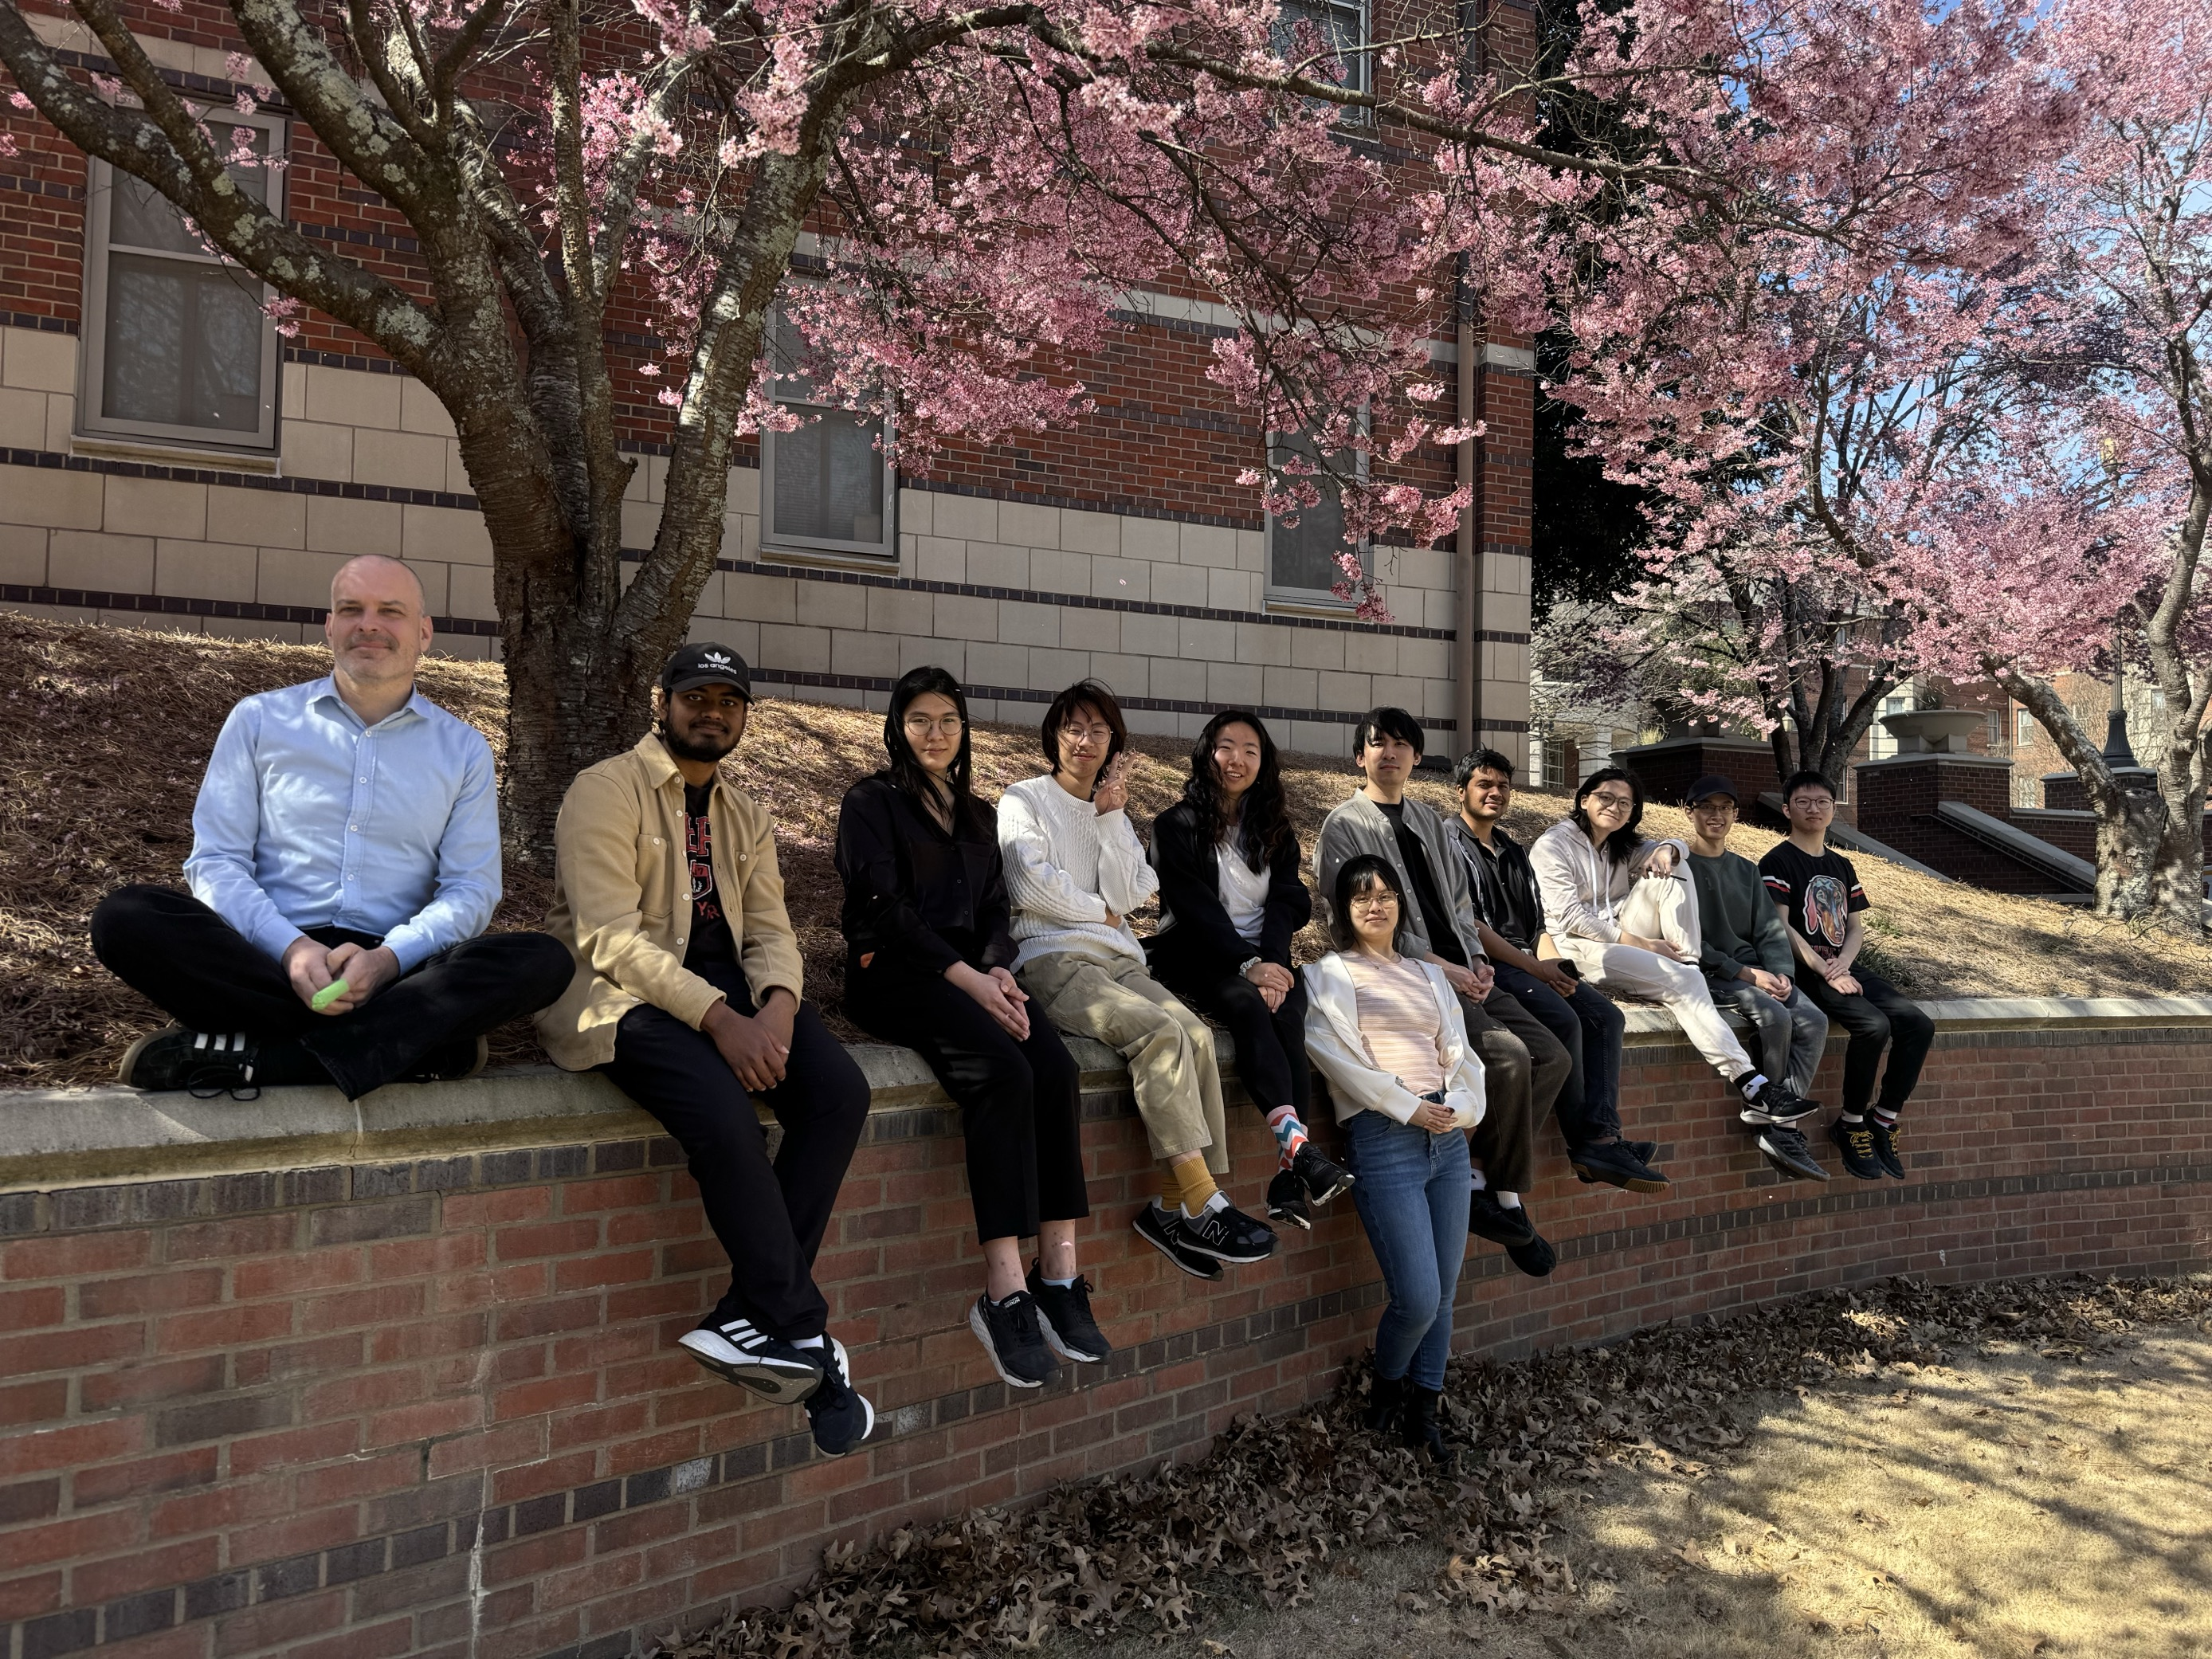
\includegraphics[width=\columnwidth]{MIG2024}%
        \end{figure}
    \end{columns}
    \addreference{\href{https://musicinformatics.gatech.edu}{musicinformatics.gatech.edu}}
    %\inserticon{person}
\end{frame}

        
    \section[areas]{areas}
        \begin{frame}{tasks}{selected tasks of interest}
            \vspace{-9mm}
            \begin{columns}
            \column{.6\linewidth}
            \begin{itemize}
                \item   \textbf{audio content analysis} \cite{lerch_introduction_2023}
                    \begin{itemize}
                        \item   music/audio \textit{classification}
                            \begin{itemize}
                                \item genre/events \cite{burred_hierarchical_2004, hung_low-resource_2023}
                                \item instruments \cite{gururani_semi-supervised_2021, chen_music_2023, ding_audio_2023}
                                \item tagging \cite{ding_audio_2023, ding_embedding_2024, ma_music_2024}
                                \item pedestrians \cite{seshadri_asped_2024, han_understanding_2024}
                            \end{itemize}
                        \item   music \textit{transcription}
                            \begin{itemize}
                                \item drum transcription \cite{wu_review_2018}
                                \item chord detection \cite{zhou_chord_2015}
                            \end{itemize}
                        \item   music \textit{performance analysis} \cite{pati_assessment_2018}
                    \end{itemize}
                 \smallskip
                 \item<2->  \textbf{audio processing}
                    \begin{itemize}
                        \item   source \textit{separation} \cite{hung_multi-task_2020, watcharasupat_generalized_2024, watcharasupat_stem-agnostic_2024}
                    \end{itemize}
                 \smallskip
                 \item<3->  \textbf{sound and music generation}
                    \begin{itemize}
                        \item   controllability \cite{pati_attribute-based_2020}
                        \item   evaluation \cite{pati_is_2021, watcharasupat_latte_2022}
                    \end{itemize}
            \end{itemize}
            \column{.4\linewidth}
            \begin{figure}
                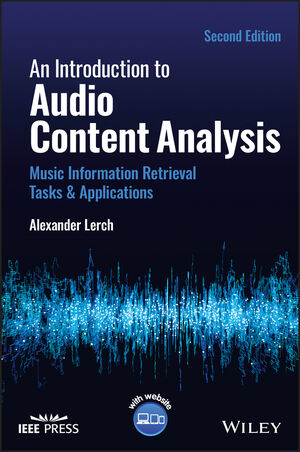
\includegraphics[scale=.20]{cover_aca2_thumb}
            \end{figure}
            \end{columns}
            \vspace{-25mm}
            \begin{flushright}
                
\includegraphics[scale=.25]{forensics}
            \end{flushright}
        \end{frame}
        
     \section[methods]{methods}
        \begin{frame}{methods}{methods of interest}
            \begin{itemize}
                \item   \textbf{representation learning}
                    \begin{itemize}
                        \item   improved structure of embedded representations \cite{seshadri_improving_2021, ma_representation_2022}
                        \item   enforcing the meaning of specific embedding dimensions \cite{pati_attribute-based_2020, pati_is_2021}
                        \item   \ldots
                    \end{itemize}
                 \bigskip
                 \item<2->  \textbf{low-resource machine learning}
                    \begin{itemize}
                        \item   semi- and self-supervised learning \cite{gururani_semi-supervised_2021, wu_labeled_2018}
                        \item   reprogramming \cite{chen_music_2023, hung_low-resource_2023}
                        \item   knowledge transfer \cite{hung_feature-informed_2022, ding_audio_2023, ding_embedding_2024}
                    \end{itemize}
                 \bigskip
                 \item<3->  \textbf{objective evaluation of generative systems}
                    \begin{itemize}
                        \item   evaluation of controllable systems with correlated attributes \cite{watcharasupat_evaluation_2021, watcharasupat_latte_2022}
                        \item   statistical models for comparison of properties \cite{yang_evaluation_2020}
                        \item   metrics for sound generation \cite{vinay_evaluating_2022}
                    \end{itemize}
            \end{itemize}
            \vspace{-40mm}
            \begin{flushright}
                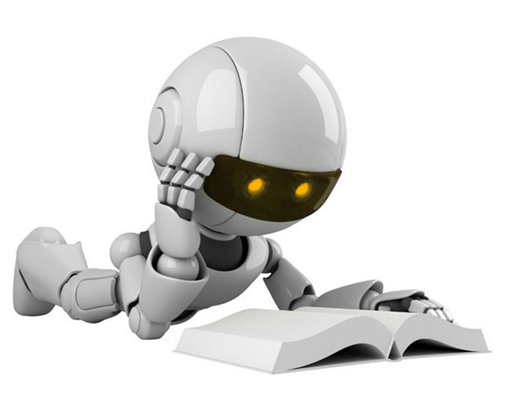
\includegraphics[scale=.20]{machinelearning}
            \end{flushright}
            \end{frame}
        
        \section[links]{thank you}

      \begin{frame}\frametitle{links}\framesubtitle{~}
            %\addreference{\href{https://github.com/alexanderlerch}{github.com/alexanderlerch}}
            \begin{block}{links}
                music informatics group:
                \href{http://musicinformatics.gatech.edu}{musicinformatics.gatech.edu}

                \bigskip
                alexander lerch: 
                    \begin{itemize}
                        \item \href{https://www.linkedin.com/in/lerch}{www.linkedin.com/in/lerch}
                        \item \href{https://github.com/alexanderlerch}{github.com/alexanderlerch}
                        \item mail: \href{mailto:alexander.lerch@gatech.edu}{alexander.lerch@gatech.edu}
                    \end{itemize}             
                %\href{http://www.alexanderlerch.com}{www.alexanderlerch.com}
                
                \bigskip                
                book: \href{https://www.AudioContentAnalysis.org}{www.AudioContentAnalysis.org}
                
                %\visible<1->{
								%\vspace{-25mm}
                %\begin{flushright}
										%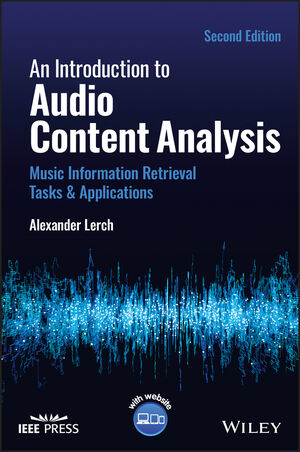
\includegraphics[scale=.20]{cover_aca2_thumb}
                %\end{flushright}
                %\vspace{-15mm}}

								%\pause
                %\bigskip
                %zplane.development: 
                %\href{https://www.zplane.de}{www.zplane.de}

                %\pause
								
								\vspace{5mm}

            \end{block}
            
			%\vspace{-22mm}
						\inserticon{mail}
            %\includegraphics[scale=.1]{wechat_qr}%
            %\begin{textblock*}{110mm}(14.25cm,7.3cm)
                %
\includegraphics[height=1.25cm,keepaspectratio]{mail}
            %\end{textblock*}            
        \end{frame}

    
    \begin{frame}[allowframebreaks]{references}{references}
    \tiny
        \printbibliography
    \end{frame}
\end{document}

